\clearpage


\section{Анализ результатов}

В этом разделе описываются результаты, полученные в настоящей работе, описываются преимущества и недостатки разработанного решения, проводится сравнение с аналогичным решением из проекта TypeChef, описываются возможные улучшения предложенного решения.

\subsection{Особенности разработанного решения}

Одним из результатов настоящей работы является модификация алгоритма Earley (см. подраздел \ref{subsec:earleymodification}), позволяющая производить синтаксический анализ для контекстно-свободных языков, используя последовательность лексем, содержащую условные ветвления, в качестве входных данных. Этот алгоритм был реализован в библиотеке для создания синтаксических анализаторов, описанной в разделе \ref{sec:parserlibimpl}. 

Для создания синтаксического анализатора, поддерживающего обработку ветвлений условной компиляции, разработчику необходимо лишь описать на предметно-ориентированном языке, предоставляемом библиотекой, грамматику используемого языка программирования. В силу поддержки библиотекой всех контекстно-свободных языков, разрабочику не придётся модифицировать грамматику языка программирования. Это выгодно отличает разработанное решение от аналогов, генерирующих LL и LR анализаторы. 

Следует заметить, что предлагаемое решение не требует от разработчиков указания синтаксических конструкций, в которых возможно наличие вершин, соответствующих точкам условного ветвления, а подразумевает возможность ветвления во всех продукциях входной грамматики. Таким образом, язык программирования описывается совершенно так же, как если бы он описывался для парсер-генератора без поддержки точек условного ветвления. 

В проекте TypeChef, например, где выбран другой подход, неудачное выделение мест ветвления может привести к сокращению количества способов использования препроцессора, а также к сложности алгоритма разбора, экспоненциально зависящей от количества точек условного ветвления.

\subsection{Сравнение с TypeChef}

В разделе \ref{sec:erlang} описывается применение разработанного решения для синтаксического анализа подмножества языка Erlang, содержащего инструкции препроцессора. В этом подразделе описывается опыт применения проекта TypeChef для создания синтаксического анализатора для того же подмножества языка Erlang, проводится эмпирическое сравнение объёма трудозатрат на реализацию решений, производительности полученных решений.

\subsubsection{Лексический анализ}

Проект TypeChef содержит в себе реализацию препроцессирующего лексера, сохраняющего информацию о ветвях условной компиляции, для языка C, а также предоставляет интерфейсы для альтернативных его реализаций. Эти интерфейсы содержат описание функциональности специфичной для препроцессора языка С, что препятствует их использованию для других языков.

Однако, часть функциональности препроцессора языка C, реализованная в TypeChef может быть переиспользована --- например, набор средств для работы с булевыми формулами, описанный в подпроекте FeatureExprLib\footnote{\url{https://github.com/ckaestne/TypeChef/tree/master/FeatureExprLib}}.

Таким образом, для реализации лексического анализаторв в TypeChef потребуется практически полностью реализовывать препроцессирующий лексер. 

Благодаря тому, что парсеры в TypeChef не имеют явной зависимости от лексеров, а используют последовательности лексем, где каждой лексеме соответствует условие её наличия, реализовывать препроцессирующий лексер <<c нуля>> не потребовалось: был реализован адаптер, позволяющий переиспользовать лексер, описанный в подразделе \ref{subsec:preprocessinglexer}

Реализация лексера, осуществляющего препроцессирование, сохраняющее ветвления условной компиляции, с помощью решения, предлагаемого в настоящей работе, также требует существенных трудозатрат, однако, выгодно отличается наличием реализации таблицы макроопределений, разрешением имён макроопределений и другой функциональности, не имеющей зависимостей от конкретного языка программирования.

\subsubsection{Синтаксический анализ}

Для реализации синтаксического анализатора разработчики TypeChef предлагают применять реализованные ими парсер-комбинаторы, описывающие возможные места появления ветвлений условной компиляции. 

При использовании этой библиотеки пришлось несколько изменить грамматику языка Erlang с тем, чтобы избавиться от леворекурсивных правил в грамматике. Леворекурсивные конструкции пришлось реализоваывать вручную --- в листинге \ref{leftassociativebinaryop} приведен код, использованный для разбора леворекурсивных бинарных операций. 

\begin{minipage}{\linewidth}
\begin{lstlisting}[caption={Реализация леворекурсивных конструкций в TypeChef},label=leftassociativebinaryop,language=Scala]
def leftAssocBop(argParser: MultiParser[Expr], 
                  opParser: MultiParser[Elem]) =
	argParser ~ repPlain(opParser ~ argParser) ^^ {
		case left ~ tail => tail.foldLeft(left) {
			case (l, op ~ r) => 
				new BinaryExpr(l, r, op.getType)
		}
	}
\end{lstlisting}
\end{minipage}

Подобных модификаций при использовании решения, предлагаемого в данной работе не потребовалось.

\subsubsection{Объём исходного кода}

Напомним, что TypeChef использует язык Scala для описания синтаксических анализаторов, в то время, как решение, предлагаемое в данной работе использует Java.

Для описания грамматики используемого подмножества языка Erlang для TypeChef понадобилось более 200 строк исходного кода, в то время, как для библиотеки, разработанной в рамках данной работы, $\sim$150 строк исходного кода.

Из этого можно заключить, что разработанное решение обладает более лаконичным синтаксисом для описания грамматики языка программирования. Любопытно также отметить, что Scala --- более выразительный язык, чем Java, и позволяет писать до двух раз более короткие программы, обладающие схожей функциональностью \cite{scalavsjava}.


\subsubsection{Производительность}

Для эмпирического сравнения производительности применялся набор входных данных, используемый для тестирования работы синтаксического анализатора, описанного в разделе \ref{sec:erlang}.

Так как для обоих решений использовался один и тот же лексический анализатор, время, затраченное на его работу, а также адаптацию результатов его работы к интерфейсам TypeChef, не учитывалось при сравнении. После запуска анализатора для каждого входного файла выполнялась сборка мусора.

\begin{figure}[h]
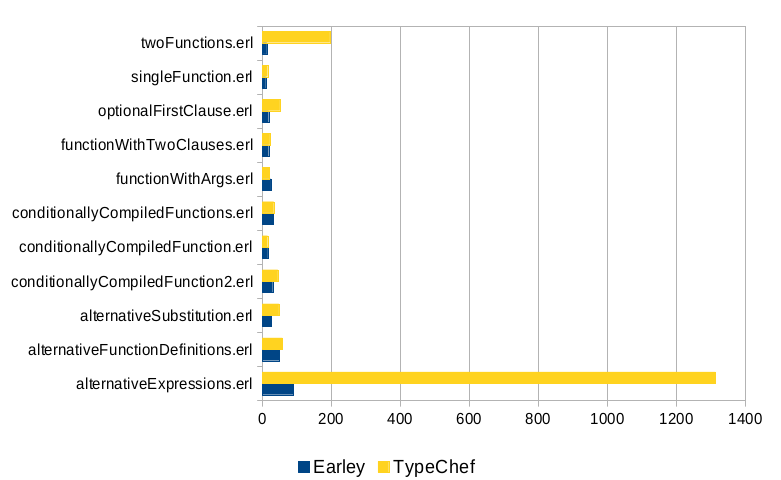
\includegraphics[width=\linewidth]{performance.png}
\caption{Время работы на тестовых данных (мс.)}
\label{chart}
\end{figure}

Из графика \ref{chart} видно, что решения показывают сравнимую скорость работы на большинстве тестов. Медианные значения составляют 25 и 45 миллисекунд для Earley и TypeChef, соответственно.

Тесты, в которых синтаксический анализатор, реализованный с помощью TypeChef, показывает значительно худшие результаты имеют следующее отличие --- в них присутствуют арифмeтические выражения с альтернативными подвыражениями --- один из таких тестов приведен в листинге \ref{altexpr}. 

\begin{minipage}{\linewidth}
\begin{lstlisting}[caption={Один из тестов с альтернативными подвыражениями},language=Erlang,label=altexpr]
-ifdef(X).
-define(EXPR, * 19).
-else.
-define(EXPR, + 18).
-endif.

foo() ->
    (11 ?EXPR) - 94.
\end{lstlisting}
\end{minipage}

Низкая скорость разбора может быть связана с неудачным описанием списочных конструкций, что приводит к экспоненциальной сложности разбора таких выражений в TypeChef.

Из вышеописанного можно заключить, что разработанное решение не уступает TypeChef в производительности, требуя при этом значительно меньших усилий при описании входного языка.

\subsection{Направления развития решения}

В этом подразделе описываются возможные направления работы связанные с улучшением решения, предлагаемого в настоящей работе, и устранением имеющихся в нем недостатков. 

На данный момент библиотека не позволяет использование в грамматике пустых правил. Известны модификации алгоритма Earley, позволяющие обрабатывать пустые правила \cite{emptyrules} --- они могут быть использованы и в модифицированном алгоритме, описанном в подразделе \ref{subsec:earleymodification}.

Выразительность предметно-ориентированного языка для описания грамматик входных языков также может быть увеличена при помощи поддержки EBNF синтаксиса.

Расширение функциональности предметно-ориентированного языка также возможно за счет применения аннотаций к правилам и за счет учета порядка их следования для разрешения неопределенностей при разборе. Это позволило бы описывать, например, грамматику выражений в интуитивно понятной форме, например, так: 

$$Expr\ ::=\ Expr\ +\ Expr\ //left-associative$$.

Модифицированный алгоритм Earley может быть улучшен при помощи обработки некоторых специальных случаев --- таких, например, как списочные структуры в грамматиках языка. На данный момент, наличие во входном тексте списка элементов, элементы которого находятся в различных ветвях условной компиляции, приводит к экспоненциальной от количества альтернативных элементов списка зависимости количества требуемой оперативной памяти и времени восстановления графа синтаксического разбора. Этого можно избежать, допуская условное вхождение элементов в списочные структуры.

Другим возможным направлением работы является разработка предметно-ориентированного языка для описания парсера и интерпретатора инструкций препроцессора --- это позволило бы существенно сократить трудозатраты на разработку синтаксического анализатора исходного кода, содержащего инструкции препроцессора.
